
\documentclass[12pt,letterpaper]{article}

% Packages
\usepackage[utf8]{inputenc}
\usepackage{amsmath}
\usepackage{amssymb}
\usepackage{graphicx}
\usepackage{float}
\usepackage{geometry}
\usepackage{hyperref}

\usepackage{listings}
\usepackage{xcolor}

\usepackage{graphicx}

\usepackage{booktabs}

\usepackage{pdfpages}

% Page margins
\geometry{margin=1in}

\begin{document}
% Document information
\begin{titlepage}
    \centering
    \vspace*{3cm}

    {\Huge\bfseries Radioactive Decay\par}

    \vspace{2cm}

    {\Large Son Thanh Truong\par}
    {\Large Student ID: 100972716\par}
    \vspace{0.5cm}
    {\large Carleton University\par}
    {\large PHYS 2007\par}
    {\large Lab Section: C\par}
    {\large Lab Partner: Lauren Gilchrist\par}
    {\large Date of Report Submission: \today\par}
    
    
    \vfill

    {\large \today\par}
\end{titlepage}



%\maketitle

\section{Introduction}

This experiment has 4 parts. Background Radiation,
The Half-Life of Barium-137m, Pb Absorption Coefficient,
and The Inverse-Square Law. In these experiments we aim
to learn about the properties of nuclear decay, and familiarize
with Geiger-Muller counters. We will measure the background
radiation in the lab room compare it with A poisson
distribution. We will determine the half-life of Barium-137m, 
an unstable isotope. We will find the absorbtion coefficient
of lead and finally we will investigate the
Inverse-Square Law.

\subsection{Background Radiation}

Background radiation is all around us, even in our physics labs.
And since we will be measuring radiation to model and fit plots,
in order to do that accurately we need to measure the background
radiation so then we could use python to subtract it from our
measurement for the best fit possible. Also the data collected
will model a Poisson distribution. The sampling was 
5 seconds per sample for 100 samples totaling to 500 seconds
for the measurement.

\subsection{The Half-Life of Barium-137m}

The goal of this part is to measure the half-life of
Barium-137m.The measurement part is almost identical to
the background radiation part. The rate of measurement is
5 seconds per sample for 240 samples totaling at 1200 seconds.
In the analysis 
using code, all of the samples were subtracted/corrected
by the average of the background radiation. Since the
total size of the number of samples aren't the same.
But more on that later.

\subsection{Pb Absorption Coefficient}
The goal of this part was to Find the absorbtion 
coefficient of lead. According to this equation:

\begin{equation}
I = I_o*np.exp(-u*x)
\end{equation}
Where $I$ is the outputed intensity
and $I_o$ is the initial intensity, 
$u$ is the absorption coefficient,
and $x$ is the thickness of the lead.
    
\subsection{The Inverse-Square Law}

Here is the equation for the Inverse-Square Law that
was given: 
\begin{equation}
I = \frac{a}{(x-b)^2} + c
\end{equation}
Where $I$ is the intensity at distance $x$ from the source,
and $a$, $b$, and $c$ are parameters to be determined.
After trying out the fit for this equation and faiing 
even after setting b and c to zero, it was decided that
b and c should be set to zero manually by using
a simpler equation:
\begin{equation}
I = \frac{a}{x^2}
\end{equation}
This was what was used to find the fit. In the end,
it only worked with this equation.

\section{Experimental Setup}

The equiptments used in this lab includes:

\begin{itemize}
    \item Geiger-Muller counter
    \item Radioactive source (Cs137, Co60)
    \item Cs-137/Ba-137m Isotope Generator
    \item Lead Plates
    \item Vernier Caliper or Micrometer
    \item Retort Stand
    \item Tongs, Petrie Dish, Paper Filter
    \item Lab Quest Mini Interface
    \item Logger Pro Software
\end{itemize}

The GM counter will be used on 
all of the 4 parts of the lab as a tool needed
to measure the radiation for all of our data.

\section{Observations}
\subsection{Background Radiation}
For this part, the GM counter was placed stationary 
with no major radiactive sources nearby. Then 100
samples of data was recorded with a duratoin of 5 seconds
per sample. Below is a sample for the data for this 
part of the lab:

\begin{tabular}{rr}
\toprule
Time (s) & Latest: Radiation (Counts) \\
\midrule
5 & 2 \\
10 & 0 \\
15 & 5 \\
20 & 0 \\
25 & 6 \\
30 & 3 \\
35 & 4 \\
40 & 3 \\
45 & 1 \\
50 & 3 \\
\bottomrule
\end{tabular}

\subsection{The Half-life of Barium-137m}
One round of continuous measurements of
5s/sample for 1200s in total. This is only a sample
of the measurement.

\begin{tabular}{rr}
\toprule
Time (s) & Latest: Radiation (Counts) \\
\midrule
5 & 245 \\
10 & 218 \\
15 & 251 \\
20 & 247 \\
25 & 234 \\
30 & 235 \\
35 & 205 \\
40 & 220 \\
45 & 221 \\
50 & 239 \\
\bottomrule
\end{tabular}

\subsection{Pb Absorption Coefficient}

There are 5 different square lead sheets of different
thinknesses. Sheets were stacked from zero sheets
to five. Each time one sample of 200s duration was 
recorded. Here is the results of all of the data gathered.
The most important colume that is being graphed is
The Thickness, and the Counts.

\begin{tabular}{rrrrrrr}
\toprule
Thickness (cm) & Counts & Average Sheet Thickness (mm) & Trial 1 & Trial 2 & Trial 3 & Minus Ziplock Bag \\
\midrule
0.000000 & 397 & 0.000000 & NaN & NaN & NaN & NaN \\
1.770000 & 361 & 1.770000 & 1.920000 & 1.890000 & 1.980000 & 0.160000 \\
5.870000 & 386 & 4.100000 & 3.770000 & 4.200000 & 4.810000 & 0.160000 \\
7.523333 & 360 & 1.653333 & 1.840000 & 1.810000 & 1.820000 & 0.170000 \\
10.136667 & 323 & 2.613333 & 2.780000 & 2.740000 & 2.770000 & 0.150000 \\
11.813333 & 270 & 1.676667 & 1.840000 & 1.840000 & 1.830000 & 0.160000 \\
\bottomrule
\end{tabular}



\section{Data Analysis}

\subsection{Background Radiation}
For the Background Radiation, we took 100 
samples of 5s duration. The result for the 
average/mean of backround radiation rate
using python's numpy library, np.mean is:
2.68 +/- 1.54 Counts per 5 seconds.
Using the python code the sample variance was given as 
2.38 $(Counts per 5 seconds)^2$. The standard deviation
is the square root of that, 1.54. Here is a graph of
the background radiation total counts in 5s versus
how many times that happened inthe Y-axis.

\begin{figure}[htbp]
    \centering
    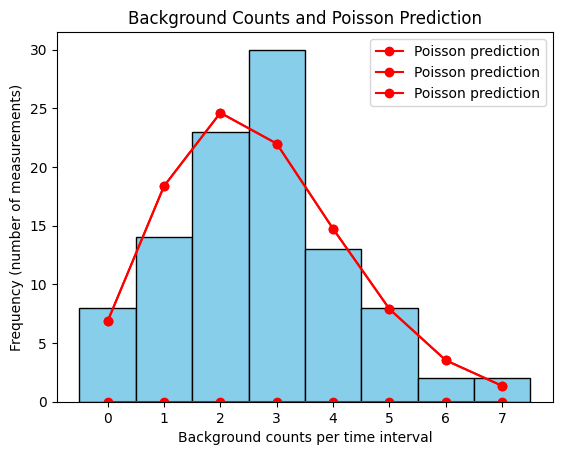
\includegraphics[width=0.8\textwidth]{Radioactive Decay Graphs/BG_histogram with Fit.png}
    \caption{Radioactive decay of Barium-137m over time.}
    \label{fig:half_life}
\end{figure}

\subsection{The Half-Life of Barium-137m}
To find the half-life of Barium-137m,
the Barium radioactive material was put very close
to The GM counter. The sample rate was 5s/sample.
When the data was analyzed, the background radiation
counts data recorded in the previous section were
subtracted easily using programming. Basically,
the mean of the Background Radiation were subtracted
from each sample. This is very easily done using
Python. Here is the line of code used to subtract the
Barium Radiation recording:

\begin{lstlisting}[language=Python]
# 5. Subtract the corrected average background
corrected_counts = HL_corrected - bkgAvg_corrected
\end{lstlisting}

There were other calibrations to correct the data for
a better fit, but the resulting change was so small
that I believe that it could be neglected but still
make a great fit. The Calibration is called Geiger
Counter Dead Time. Here is the equation for that:
\begin{equation}
N_{true} = \frac{n_{observed}}{1 - n_{observed} \tau}
\end{equation}
$N_{true}$ is the true count, 
$n_{observed}$ is the observed count, 
and $\tau$ is the dead time of the Geiger counter.

After subtracting the background radiation,
The data was plotted and here it is:
\begin{figure}[htbp]
    \centering
    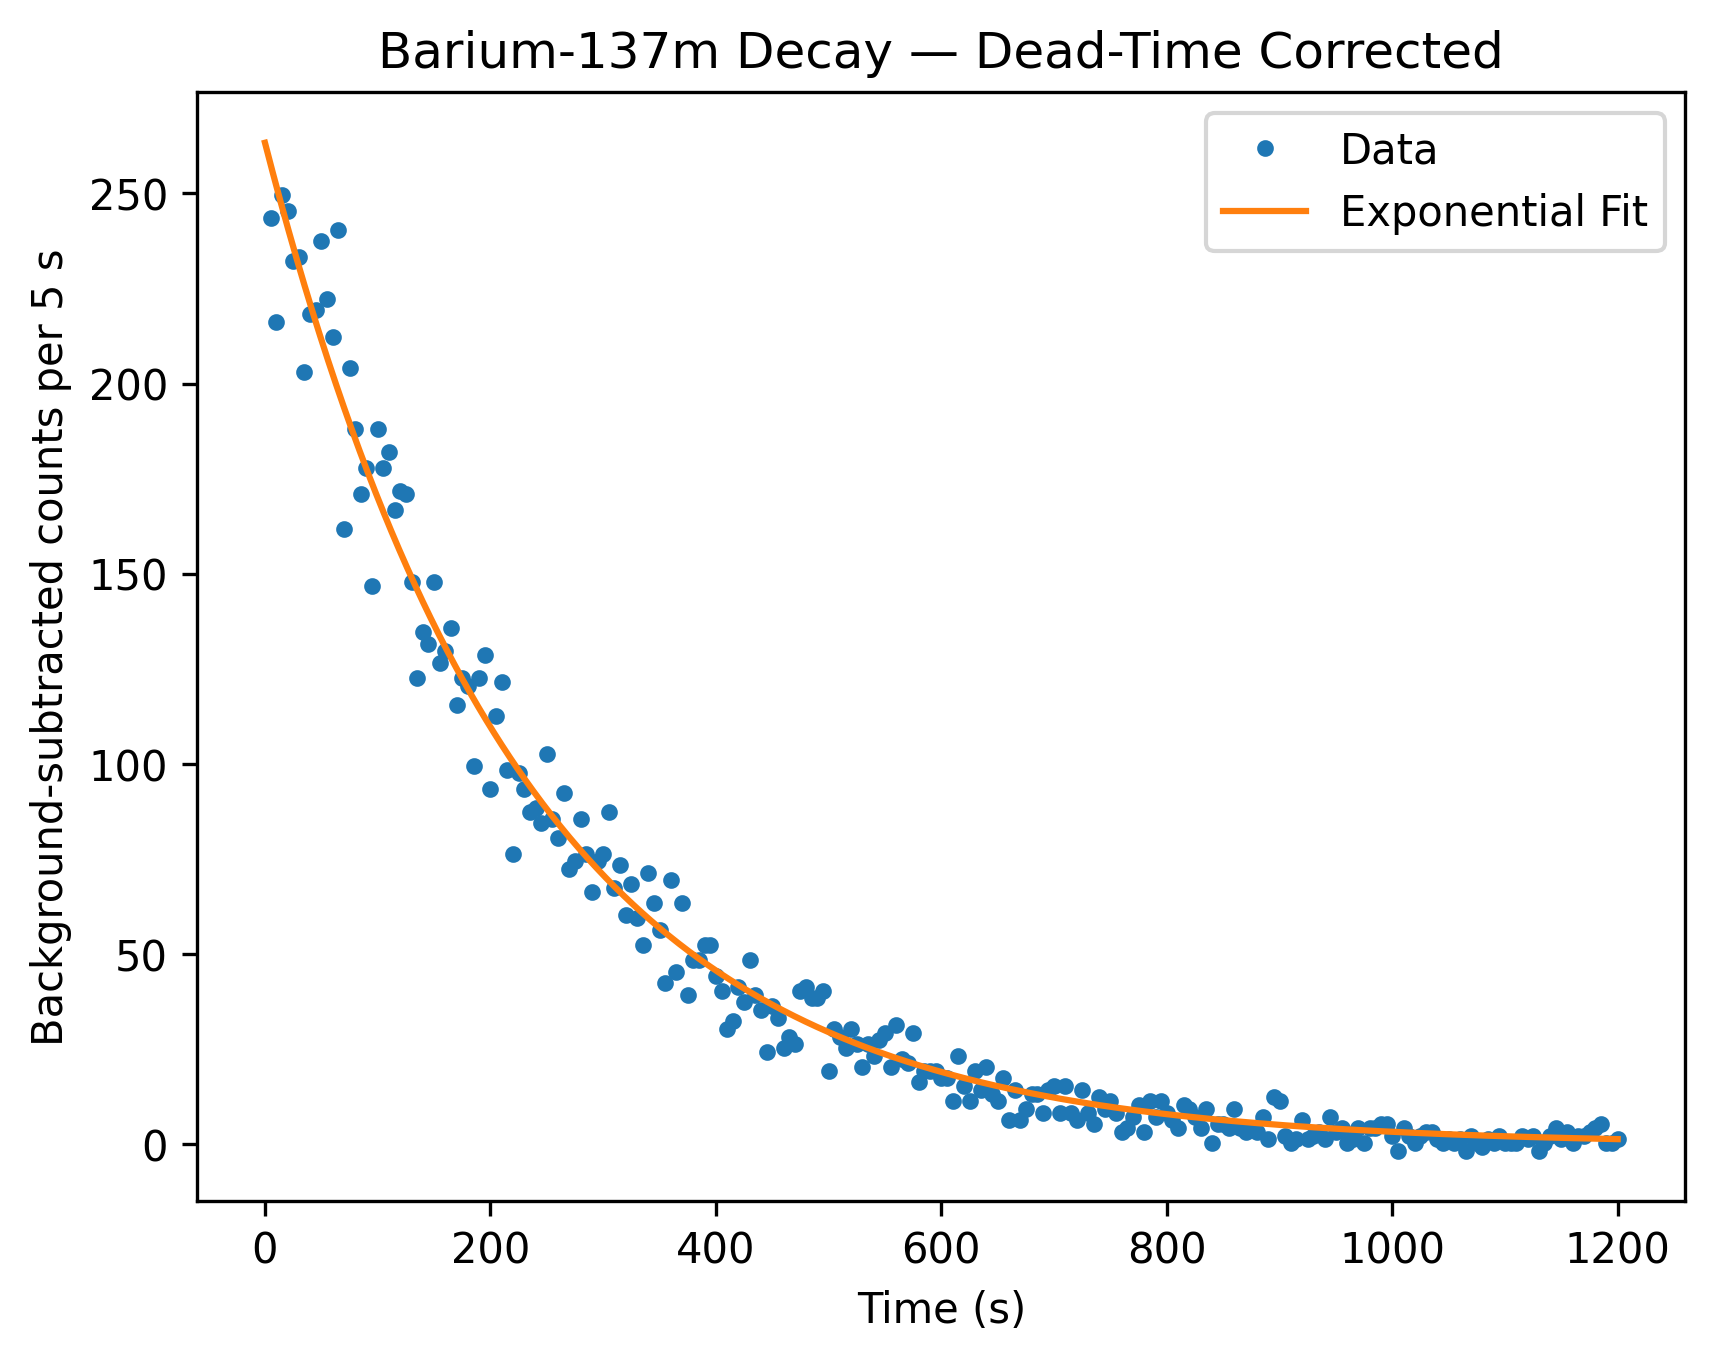
\includegraphics[width=0.8\textwidth]{Radioactive Decay Graphs/Half-Life of Ba with Fit.png}
    \caption{Radioactive decay of Barium-137m over time.}
    \label{fig:half_life}
\end{figure}
The half-life of Barium-137m is:
Half-Life = ln2/lambda = ln2/0.0043773832515909585 is approximately 158.35 seconds
For the error calculation:
\begin{equation}
\sigma_{T_{1/2}} =
 |\frac{dT}{d\lambda}| \sigma_\lambda =
 |\frac{d(ln2/\lambda)}{d\lambda}|\sigma_\lambda =
|-ln2/\lambda^2| \sigma_\lambda
\end{equation}
where $\sigma_{T_{1/2}}$ is the error in the
half-life and $\sigma_\lambda$ is the error 
in the decay constant.
When the Lambda is 0.0043773832515909585 and the error
on lambda is 5.76137806e-05,we get:
\begin{equation}
\sigma_{T_{1/2}} = |-ln2/0.0043773832515909585^2| 5.76137806e-05 =
2.04812 \text{ s}
\end{equation}
The final answer is: $T_{1/2} = 158.35 \pm 2.05 \text{ s}$
\subsection{Pb Absorption Coefficient}
This part is composed of changing the thickness of
the lead that the radiation has to go through and 
measuring what that effect has on the intensity
of the radiation.
The lead involved composes of different
square sheets with different thicknesses
but average about 1mm in thickness in zip lock bags.
The data was them collected, graphed and fitted.
Below is the fitted graph showing the data points
and the fitted curve. The result is that the
absorption coefficent is 0.02 +- 0.005 cm$^{-1}$.
The error on the coefficient was exported through
the variable `pcov` from the curve fit.
\begin{figure}[htbp]
    \centering
    \includegraphics[width=0.8\textwidth]{Radioactive
    Decay Graphs/Lead Absorbtion with Fit.png}
    \caption{Pb absorption coefficient measurement.}
    \label{fig:pb_absorption}
\end{figure}

\subsection{Inverse-Square Law}
The analyis for the Inverse-Square Law is very
similar to previous analysis. After data is collected
during the experiment, the data was sampled into 
a one dimensional array. Two arrays of the same size
were created for graphing. The Background mean
was used for correction. At that point the Curve Fit
function was used. The initial function from the lab
manual that I tried was:

\begin{lstlisting}[language=Python]
    def ISL(x,a,b,c,n):
        return a/(x-b)**n + c
\end{lstlisting}
After calling Curve Fit many times with no luck
even after setting b, and c to zero in the call.
I decided to set them to zero manually by removing
them out of the equation.
The new function I used was:
\begin{lstlisting}[language=Python]
def ISL2(x,a,n):
        return a/x**n
\end{lstlisting}

Then I called:

\begin{lstlisting}[language=Python]
popt, pcov = curve_fit(I, thickness, Counts, [1])
\end{lstlisting}

Where the very last parameter [1] is my
guess for N. I ended up getting N = 1.53.
The error on N is 0.0558.
Thus the total result is $N = 1.53 +/- 0.0558$.
\begin{figure}[htbp]
    \centering
    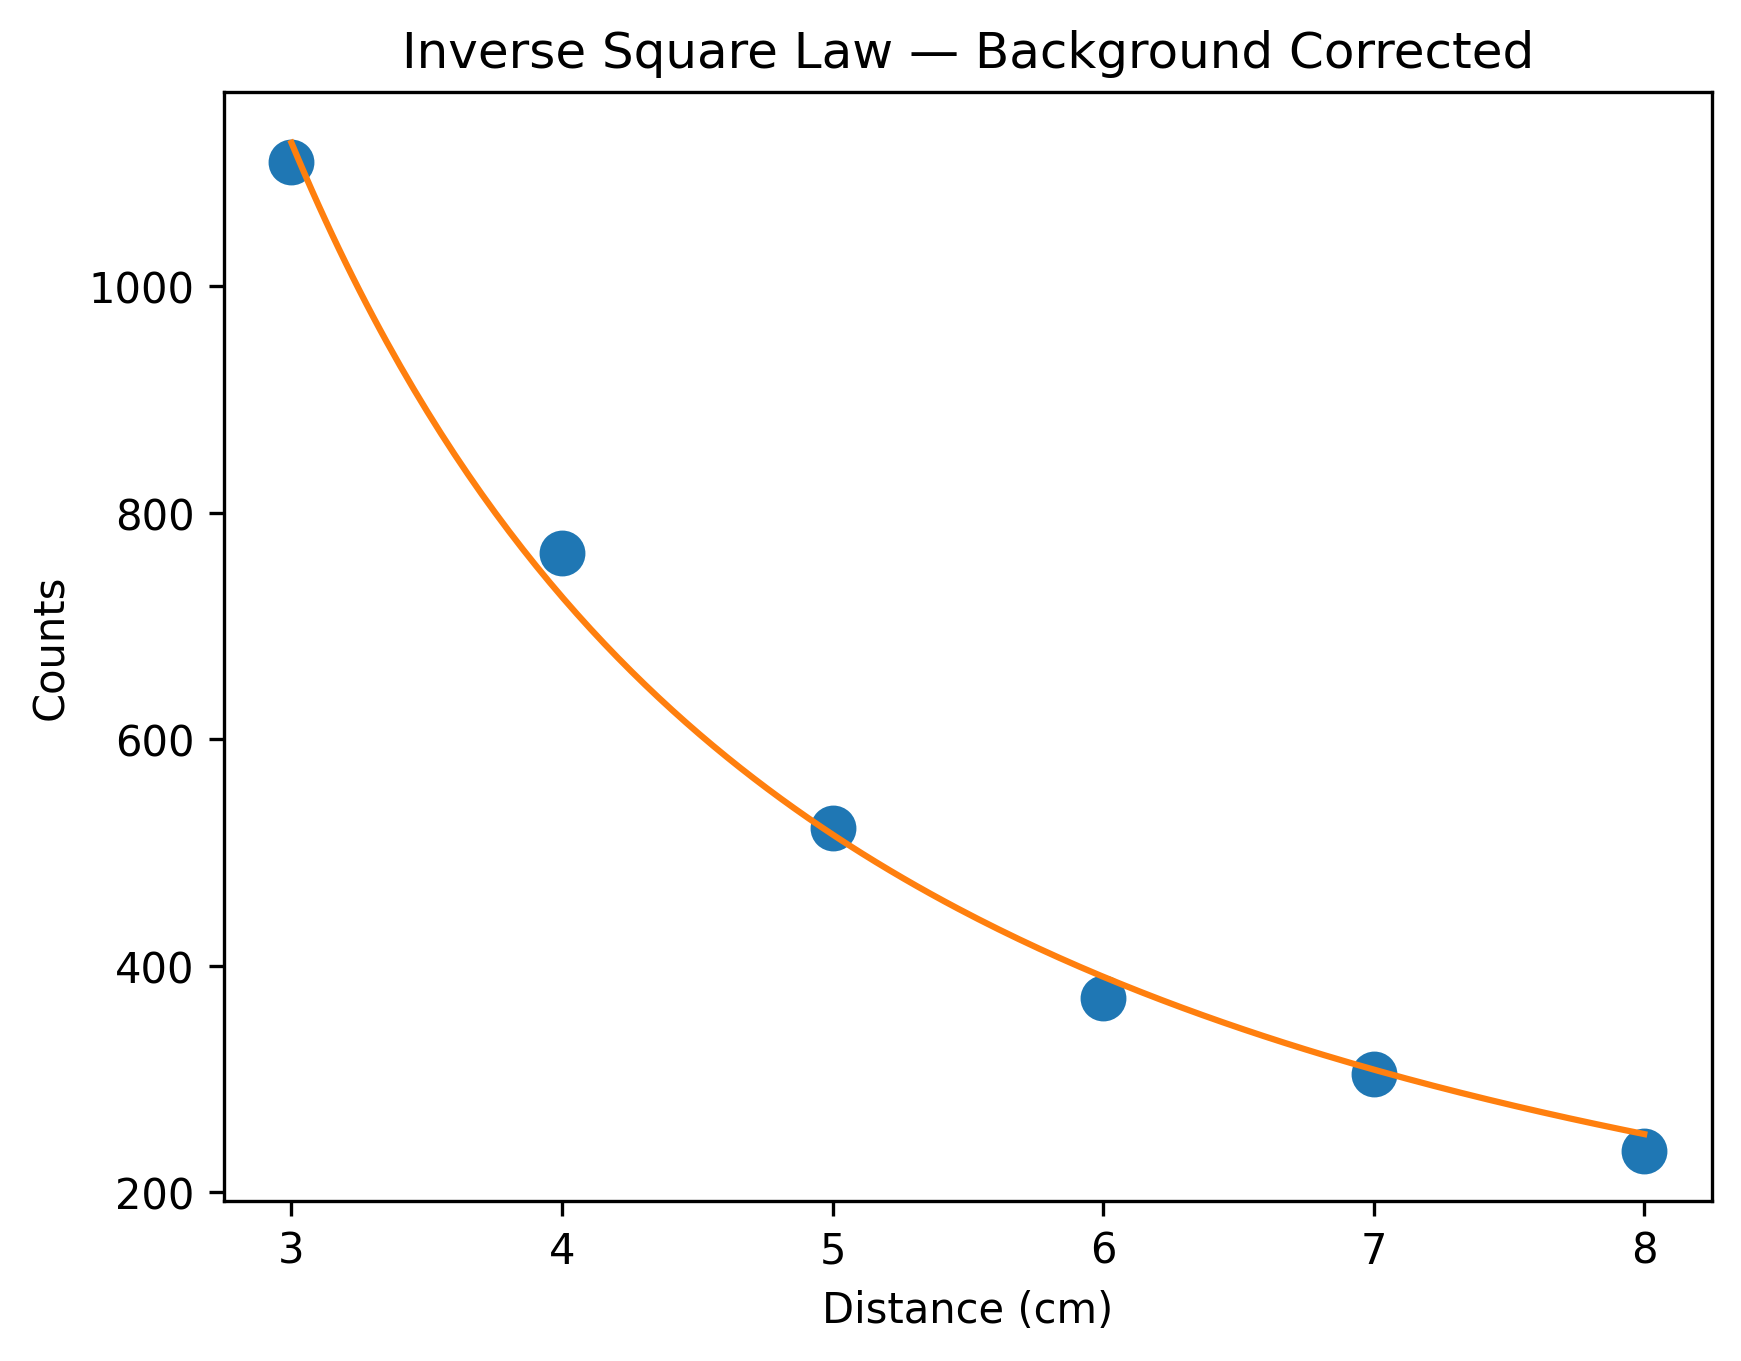
\includegraphics[width=0.8\textwidth]{Radioactive Decay Graphs/Inverse Square Law with Fit.png}
    \caption{Inverse-square law measurement.}
    \label{fig:inverse_square}
\end{figure}



\section{Discussion}
The results of this lab are as follows: with the
background radiation part of the lab, it was graphed
the data using bins and it seems like it does look
like a poisson distribution when comparing. The mean
for this data set is 2.68 +/- 1.54 Counts per 5 seconds.

With the half-life calculation, the final value, the
half-life of this process is:
158.35 +/- 2.05 seconds.
That's reasonably good, considering the accepted
value is 153.12 seconds.

Part 3 the Lead Absorption Coefficient was: 
$0.02 +/- 0.005 mm^{-1}$ = $0.2 +/- 0.05 cm^{-1}$
The expected value should be $1.26 cm^{-1}$. So something
went wrong there, I wonder if we switched cm for mm.
Because everything is measured in mm, but the
final value is cm. This is a lesson for me for next
time for sure.


And the final part, the Inverse-Square Law's N constant
is: $1.53 +/- 0.0558$
N should be 2, but it's calculated to be 1.53. the 
biggest source of error I see here is that I actually
used a 20 cm ruler to match distances with the one
meter ruler which is very imprecise. I was in a hurry
to get it done before time ran out. I should've put on
my mask, stay more calm to make way better measurements.


Overall, I felt very successful and optimistic with 
this lab because the results seem to be very accurate.
because all the errors are very low. I wonder if's it
because I was the only one taking measurements for 
some of the parts. I'm
slower than my lab partner but I'm actually very careful
and I do things in order and with precision. When my lab
partner came I had already finished taking data. Data
for our other labs were never this precise, there were
multiple problems with the data and the fits
doesn't look good. I guess it pays to be slow and 
careful.

In the next lab, I will try to understand the theory
beforehand so I wouldn't be so confused meaning I could
resolve my partner's question and not have to rely on
 our busy TAs. Also on another note, the use of masks
 seems to lower my anxiety by quite a lot. I was able
 understand our professor better when he lectures, be
 more focused during the experiment and have way more
 mental stamina. Masks are the way to go.


\section{Excel/Jupyter Files}




\clearpage
\appendix

\section{Experimental Data}

\section{Background Radiation Data}
\label{app:background}
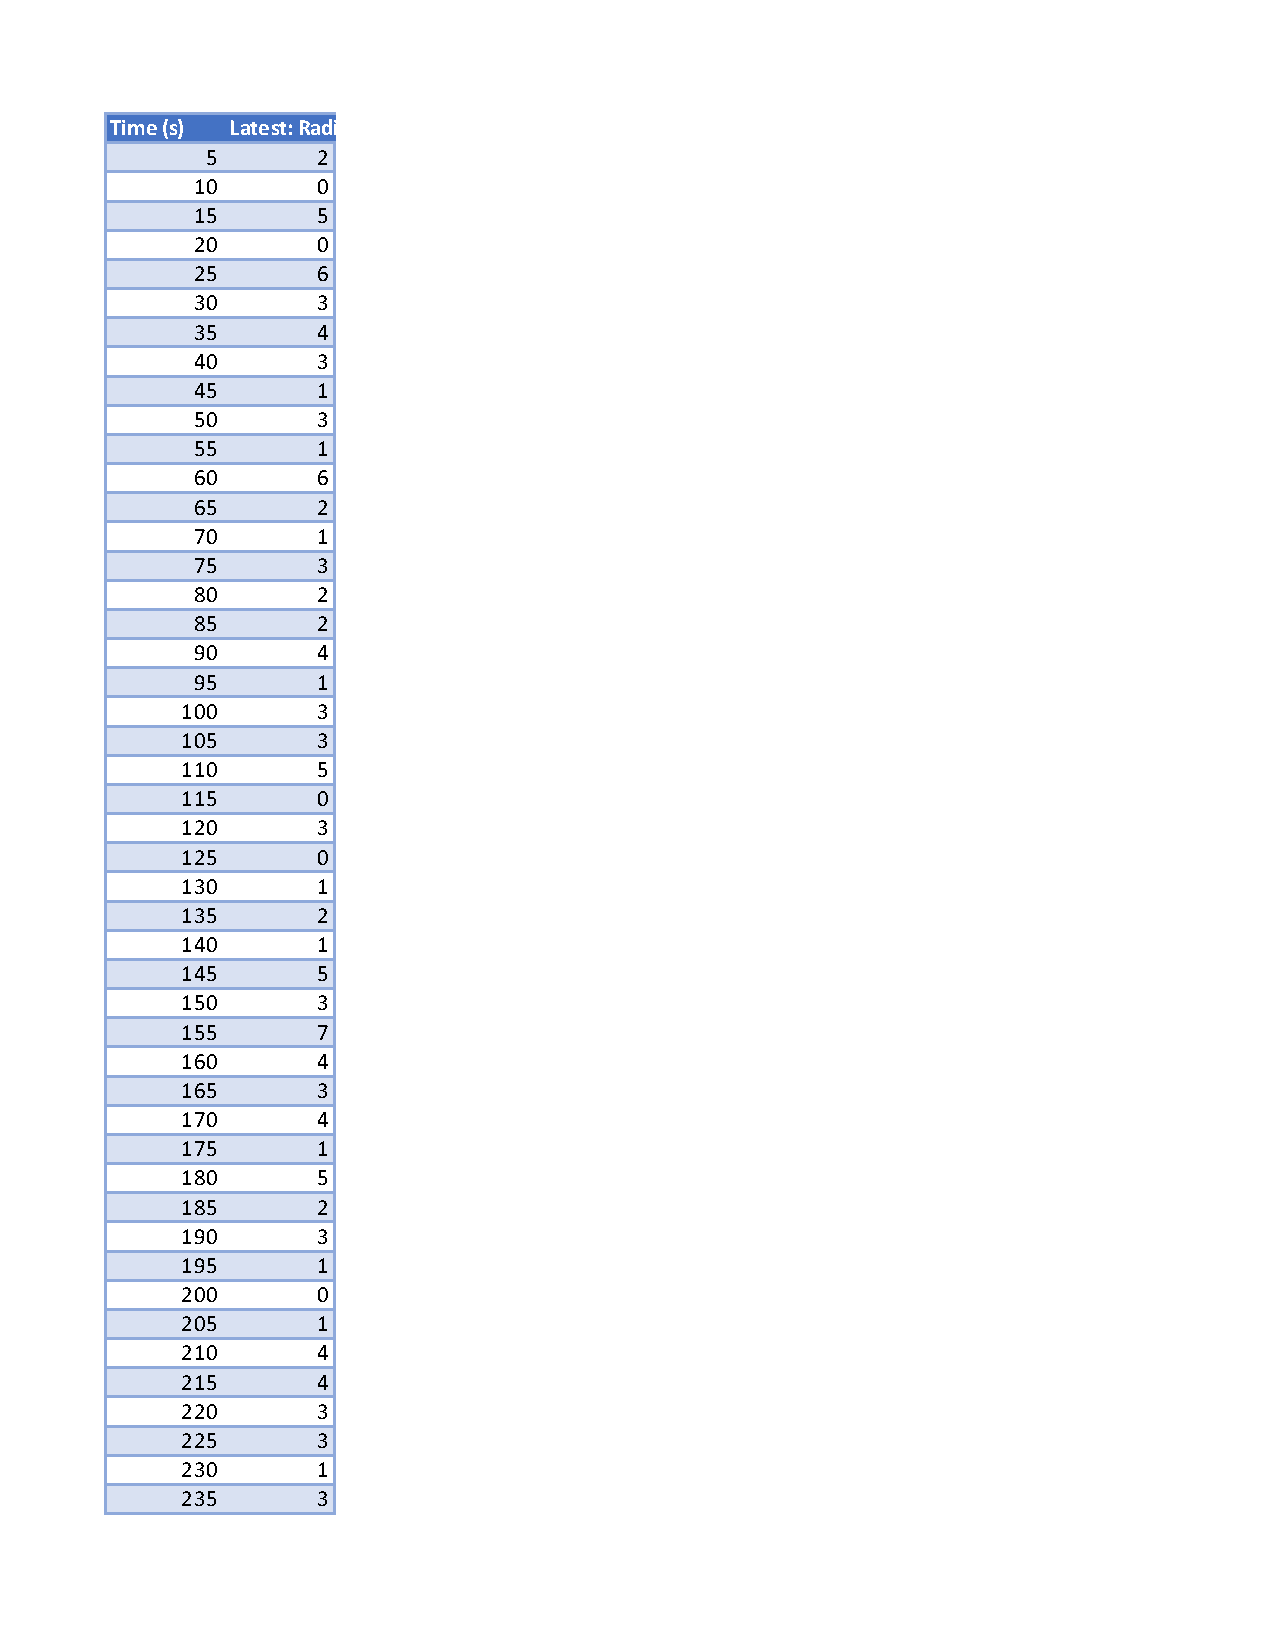
\includepdf[pages=-]{Background Table.pdf}

\section{Barium-137m Half-Life Data}
\label{app:halflife}
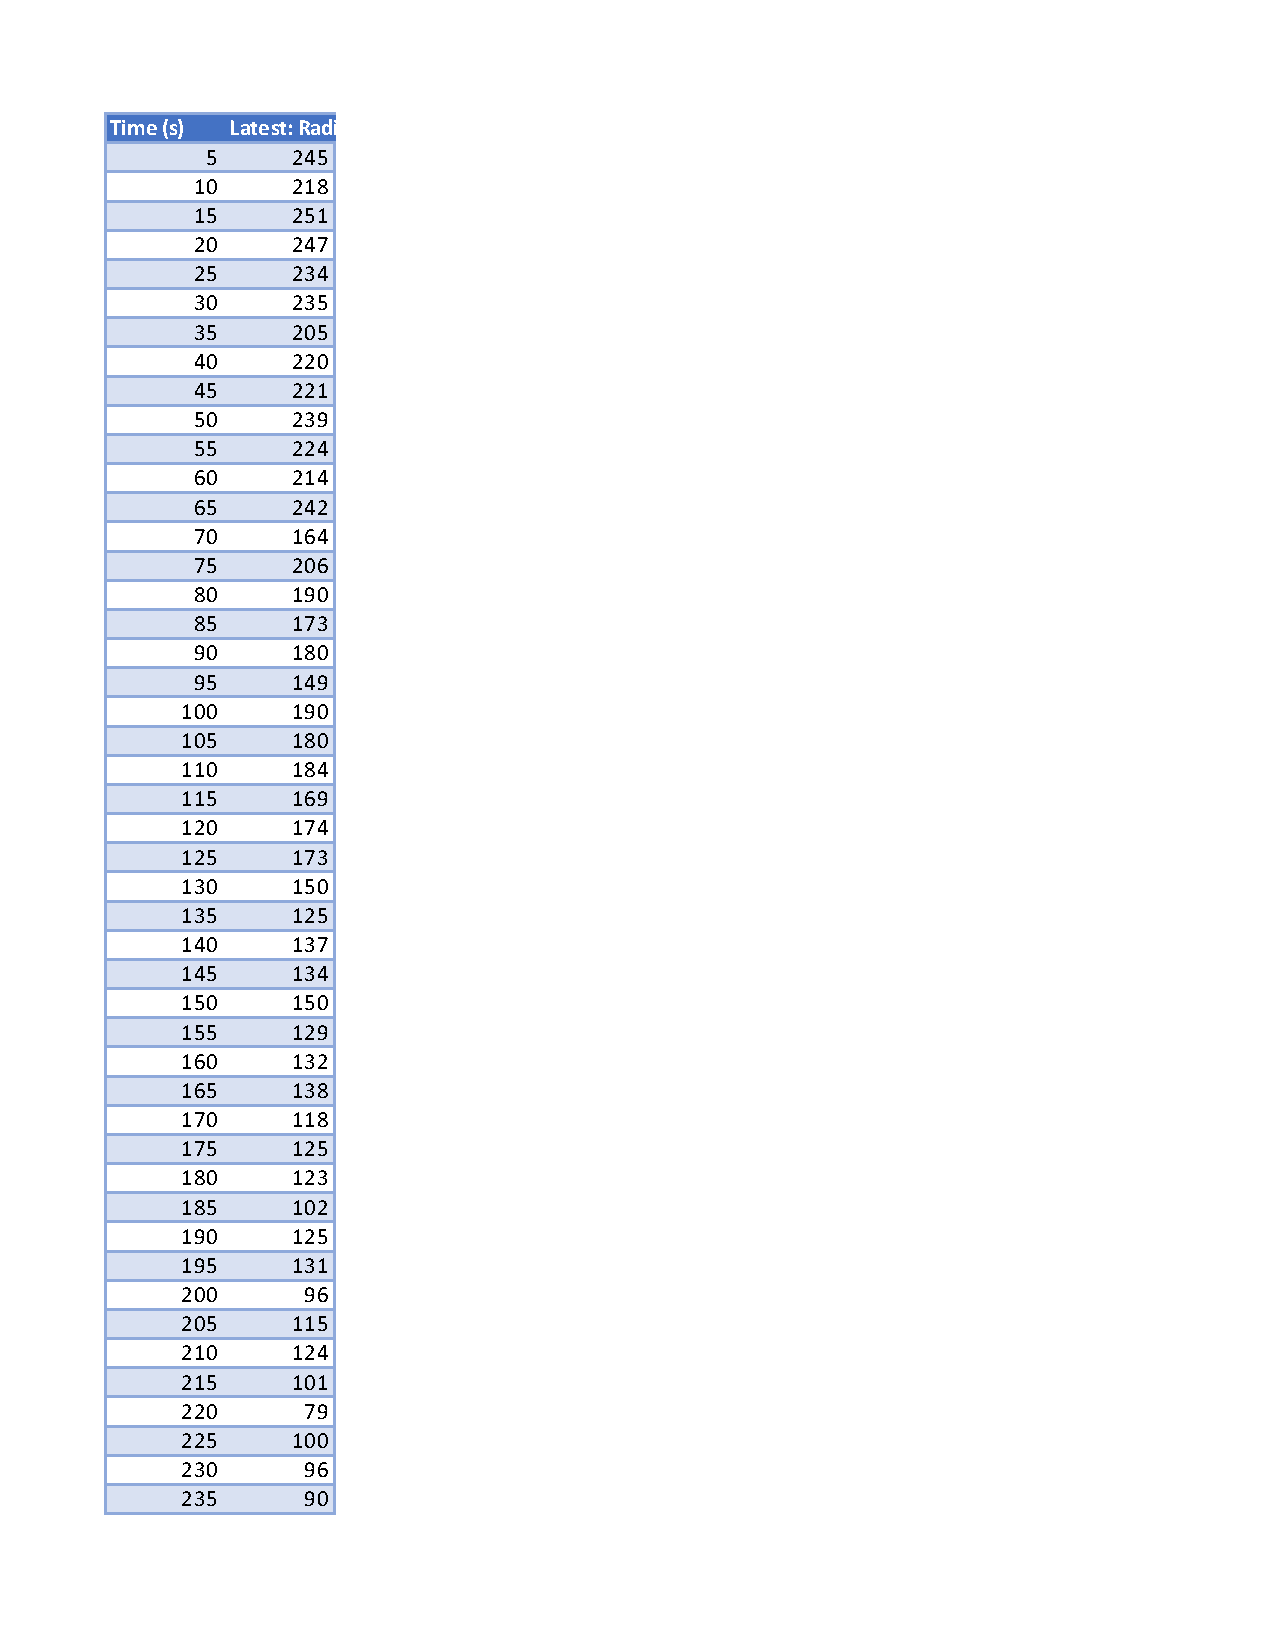
\includepdf[pages=-]{Half-Life Table.pdf}

\section{Lead Absorption Data}
\label{app:lead}
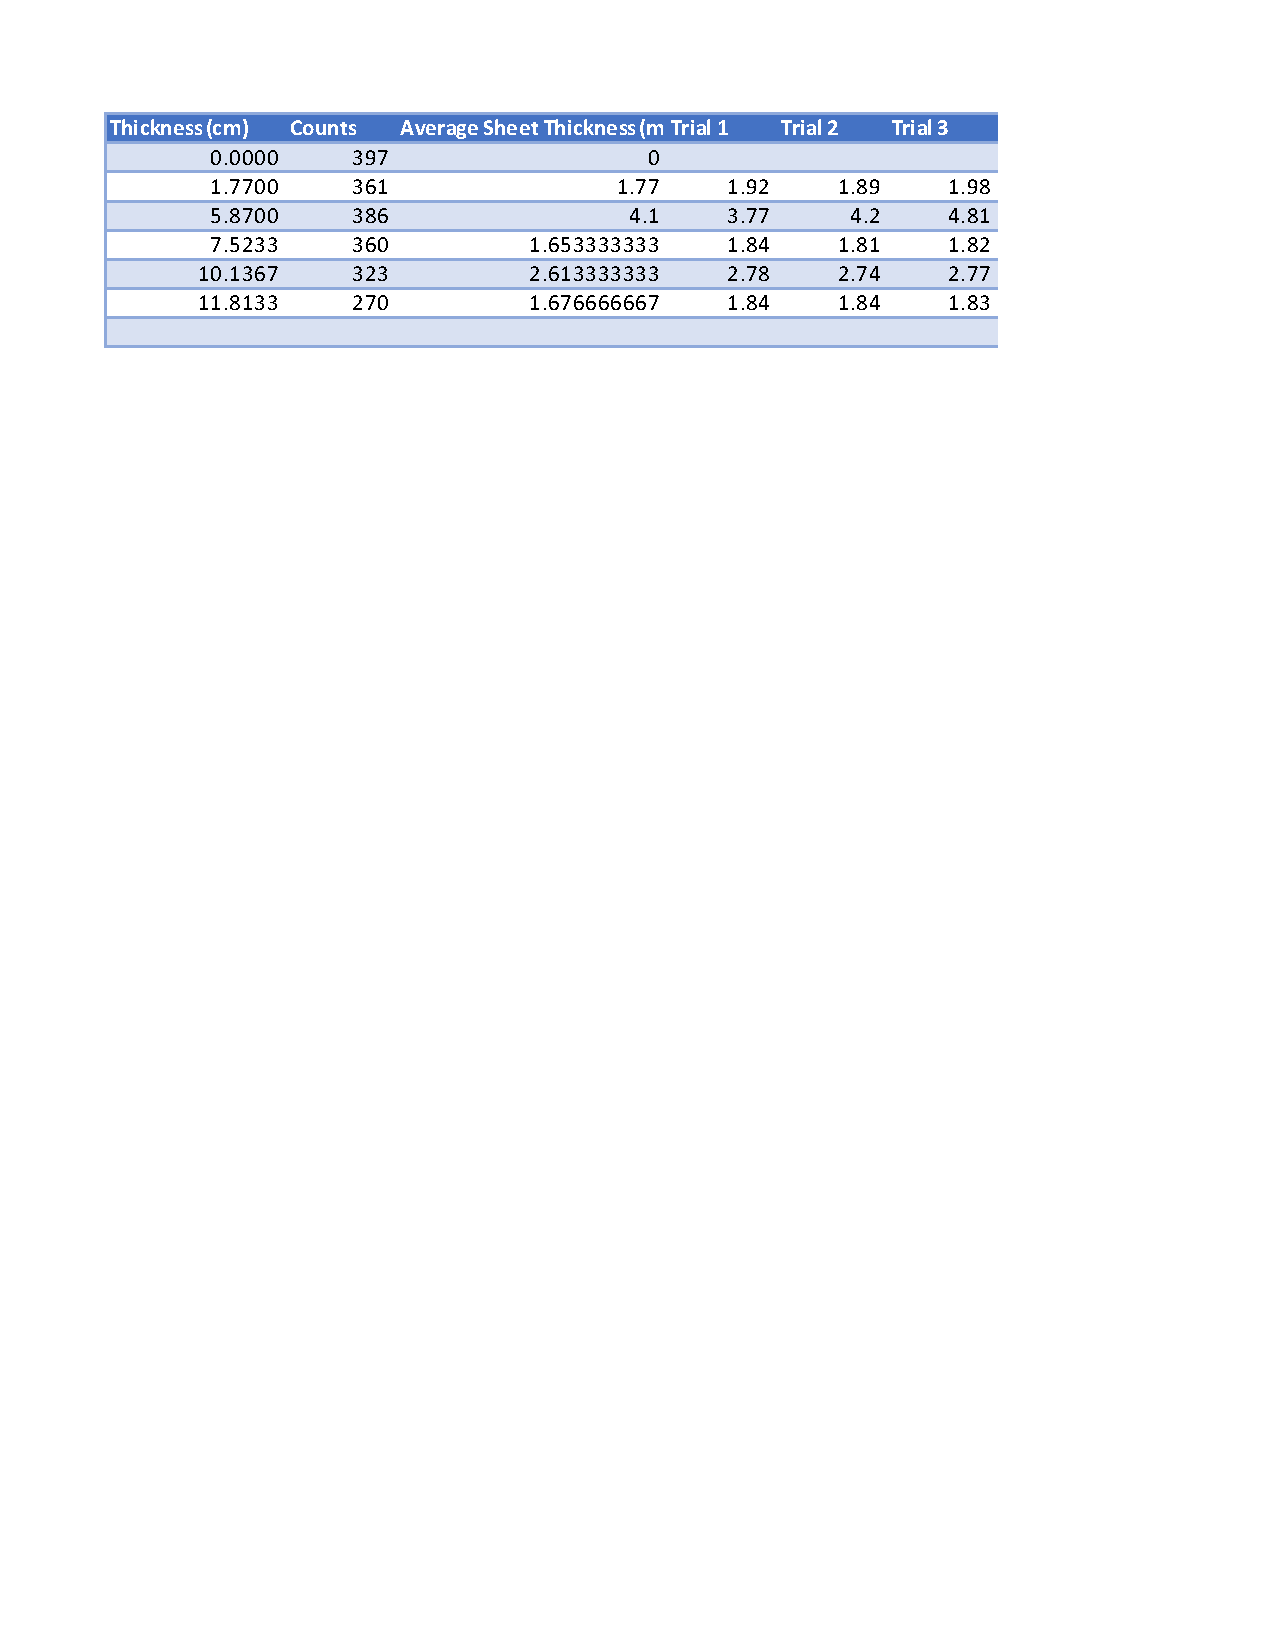
\includepdf[pages=-]{Absorption Coefficient Table.pdf}

\section{Inverse Square Law Data}
\label{app:inverse}
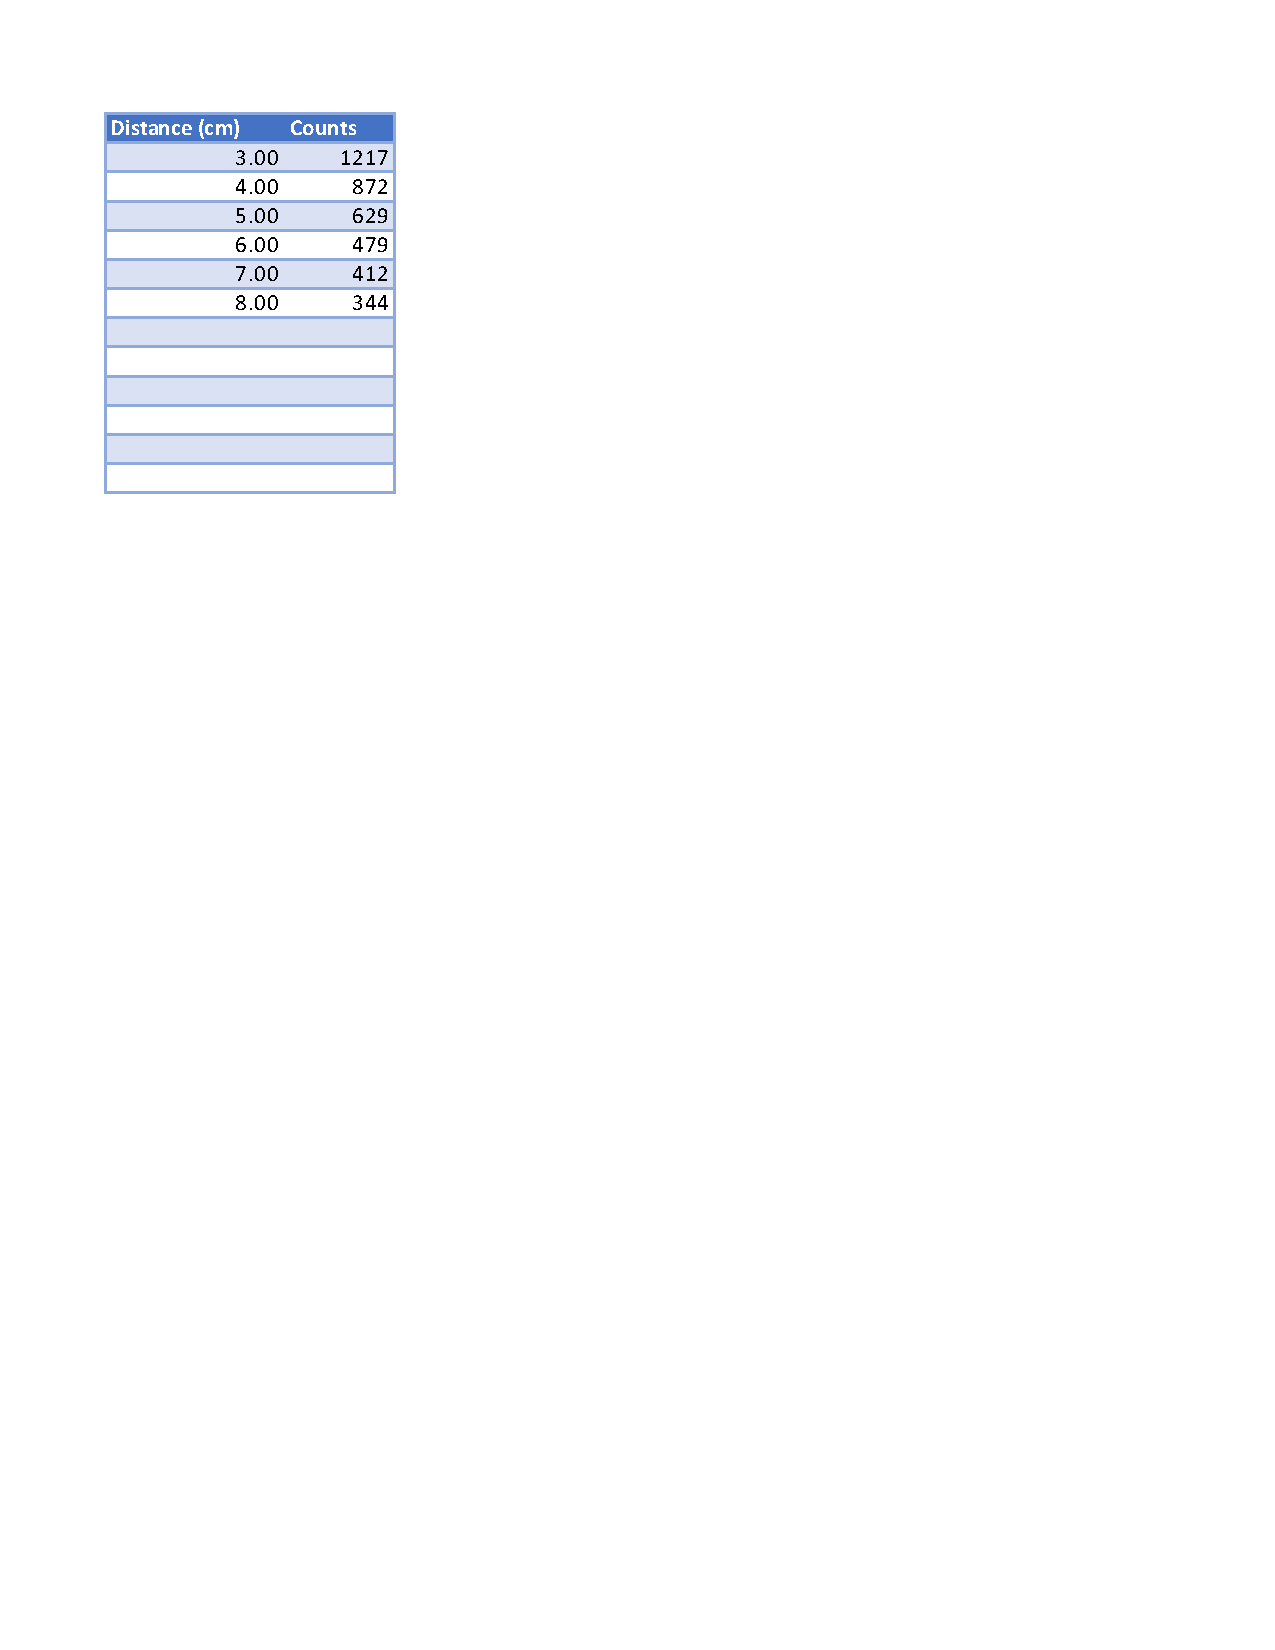
\includepdf[pages=-]{ISL Table.pdf}


\clearpage
\section{Python Code}

% Complete Jupyter Notebook
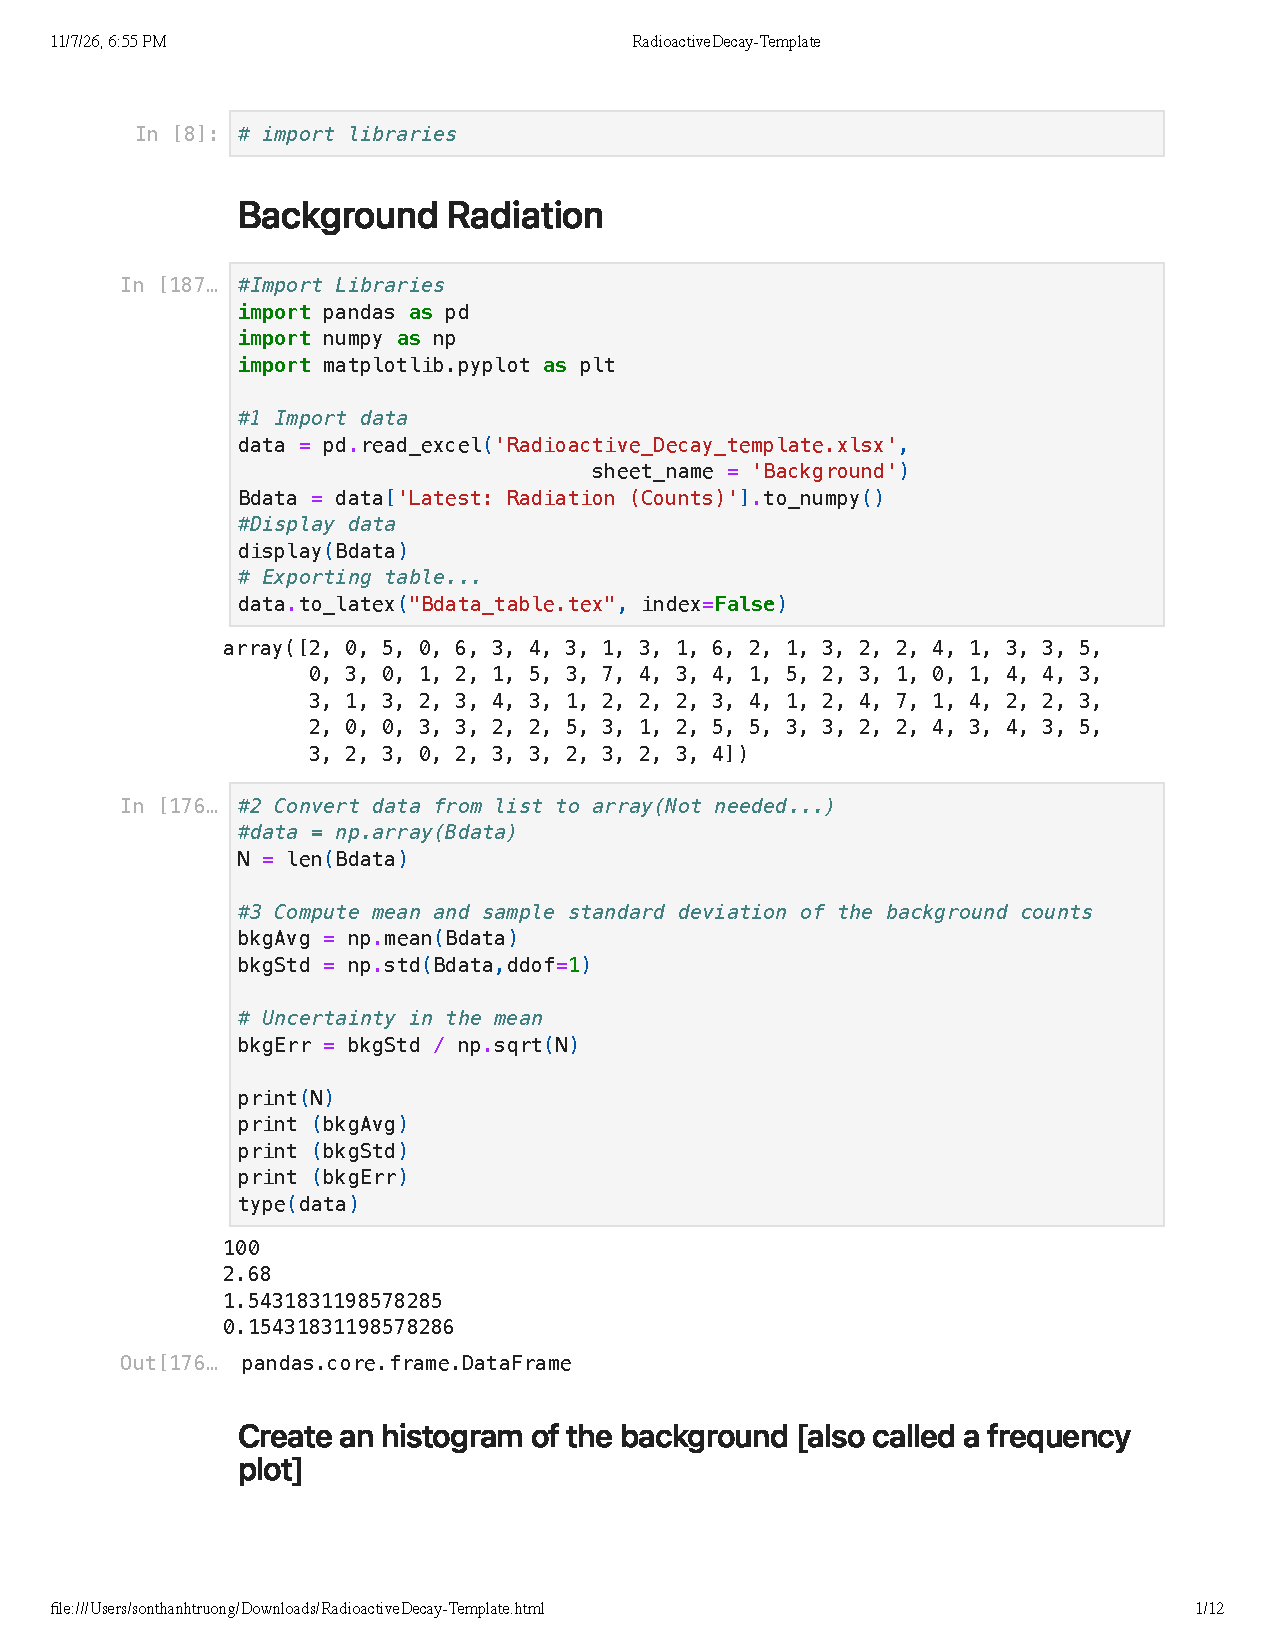
\includepdf[pages=-]{RadioactiveDecay-Template.pdf}





\clearpage
\appendix



\end{document}
